\documentclass[a4paper,11pt]{report}

\usepackage{ucs}
\usepackage[utf8]{inputenc}
\usepackage{babel}
\usepackage{fontenc}
\usepackage{graphicx}

\usepackage[dvips]{hyperref}

\author{William Burbidge}
\date{11/07/2022}

\begin{document}

\end{document}
\documentclass[a4paper,11pt]{report}

\usepackage[a4paper, total={6.8in, 9.8in}]{geometry}

\usepackage[utf8]{inputenc}

\usepackage{setspace}

\usepackage{subfigure}

\usepackage{gensymb}

\usepackage{todonotes}

\usepackage{hyperref}

\usepackage{fancyhdr}

\pagestyle{fancy}

\cfoot{WACL Electronics Course}

\fancyfoot[R]{\thepage}

\usepackage{graphicx}

\graphicspath{ {./images/} }

\setlength{\parindent}{0pt}

% Title Page

\title{WACL Electronics Course}

\author{William Burbidge}

% Create the command used for questions

\newcommand{\Theory}[1] % This is what you will use to create a new question

{

% \par\noindent % Creates a new unindented paragraph

\phantomsection % Needed for hyperref compatibility with the \addcontensline command

\todo[inline, color=green!30]{\textbf{#1}} % Uses the todonotes package to create a fancy box to put the question

\vspace{1em} % White space after the question before the start of the answer

}

% Create the command used for questions

\newcommand{\Examples}[1] % This is what you will use to create a new question

{

\par\noindent % Creates a new unindented paragraph

\phantomsection % Needed for hyperref compatibility with the \addcontensline command

\todo[inline, color=red!30]{\textbf{#1}} % Uses the todonotes package to create a fancy box to put the question

\vspace{1em} % White space after the question before the start of the answer

}

% Create the command used for questions

\newcommand{\Simulation}[1] % This is what you will use to create a new question

{

\par\noindent % Creates a new unindented paragraph

\phantomsection % Needed for hyperref compatibility with the \addcontensline command

\todo[inline, color=yellow!30]{\textbf{#1}} % Uses the todonotes package to create a fancy box to put the question

\vspace{1em} % White space after the question before the start of the answer

}

% Create the command used for questions

\newcommand{\Quiz}[1] % This is what you will use to create a new question

{

\par\noindent % Creates a new unindented paragraph

\phantomsection % Needed for hyperref compatibility with the \addcontensline command

\todo[inline, color=blue!30]{\textbf{#1}} % Uses the todonotes package to create a fancy box to put the question

\vspace{1em} % White space after the question before the start of the answer

}

\usepackage{parskip}

\begin{document}

\maketitle

\tableofcontents

\doublespacing

% \begin{singlespace} \end{singlespace} may be needed for example in bibleography%

\pagebreak

\section{Electronics Fundamentals}

Understanding the electronics behind processes or sensors used in the field can help to optimize time, reduce costs and find tailored solutions to problems within research. Whether this is in the repair of equipment, design of a simple system to automate data measurement or to help explain why some read data differs significantly from expected.

This course will take you through the basics, all while linking it to examples important for chemistry and Atmospheric related research. By the end of the course, you should understand basic electronics theory and practice, a knowledge of terminology used, and should be able to build a basic system using a sensor and control loop.

There will be an opportunity to learn theory, to see how this relates to practice, often with chemistry specific examples, and the chance to use and view simulation to help to consolidate knowledge. Then, as your confidence grows, you will put this learning into practice.

The course will also touch upon a range of areas that are useful to be aware of when dealing with electronics, such as enclosures, environmental factors, sourcing parts and safety. Where it would be beneficial, there will be references to chemistry theory, to provide another way of looking at some theories, likely more familiar to you. We will start with the basics of electronics. There is a range of ways to represent this. In this case, we will start with the physics, using analogies along the way.

Electronics involves a flow of electrons, for a transfer of energy over time (i.e. power). This is represented through voltage and current, often seen as the key units of electricity. If this was to be represented as letters within a mail network, voltage is the magnitude/ number of letters each mail person carries, where current is the rate at which a new batch is delivered/ how regularly they come. A component or drop-off point along the network will have a resistance, which is the number of letters they will pick up from each mail person.

From a physics standpoint, electronics works through the transfer of electrical energy, which goes through a conversion process in components. A resistance will cause a heat conversion/heat loss, where capacitance and inductance, discussed in further later on, are because of conversion to electric potential and magnetic potential.

Focusing just on resistance and power, for now, this can be represented as several key physics equations, important for physics-based electronic theory and practice.

\[V=IR , P=IV , P=I^2R , P=E/T\]

As can be seen, $P=I^2R$ can be derived by rearranging and putting $V=IR$ into $P=IV$. This can be seen below-

\[V=IR \Longleftrightarrow P=IV\]

\[P=I(IR)\]

\[P=I^2R\]

Voltage is represented with V, with the unit Volt. Current is represented with I, with the unit Ampere (Amp). Resistance is represented with R, with the unit Ohm (with the Greek letter $\ohm$). Power is represented with P, with the unit Watt. Time is represented with T and is usally in seconds.

Now the basics have been covered, a small quiz might be helpful to consolidate knowledge.

\Quiz{Quiz}

1. What does resistance demonstrate?

a) The rate of flow of electrons.

b) The energy in each “packet” or electron.

c) Conversion of electrical to thermal energy/ heat.

2. Demonstrate how you would go from the equation $P=I^2R$ to $P=IV$.

\subsection{Series and Parallel}

You can wire a circuit with parallel and series elements. A series circuit has a single loop, with components connected one after another, sharing a single voltage. A parallel circuit can have more than one loop branching out, with each loop having a voltage equivalent to the input, and the current will be split between them, based on their resistance.

Therefore, the voltage in a series loop will be distributed based on the voltage ratios. An example being, if there is a 10ohm resistor and a 5ohm resistor, where 9v is travelling through the loop, there would be a voltage drop of 6v through the 10 ohm resistor and a drop of 3v through the 5ohm resistor. With a total resistance of 15ohm, we can calculate the current to be $V=IR$, $I=V/R$, $I=9/15=0.6A$.

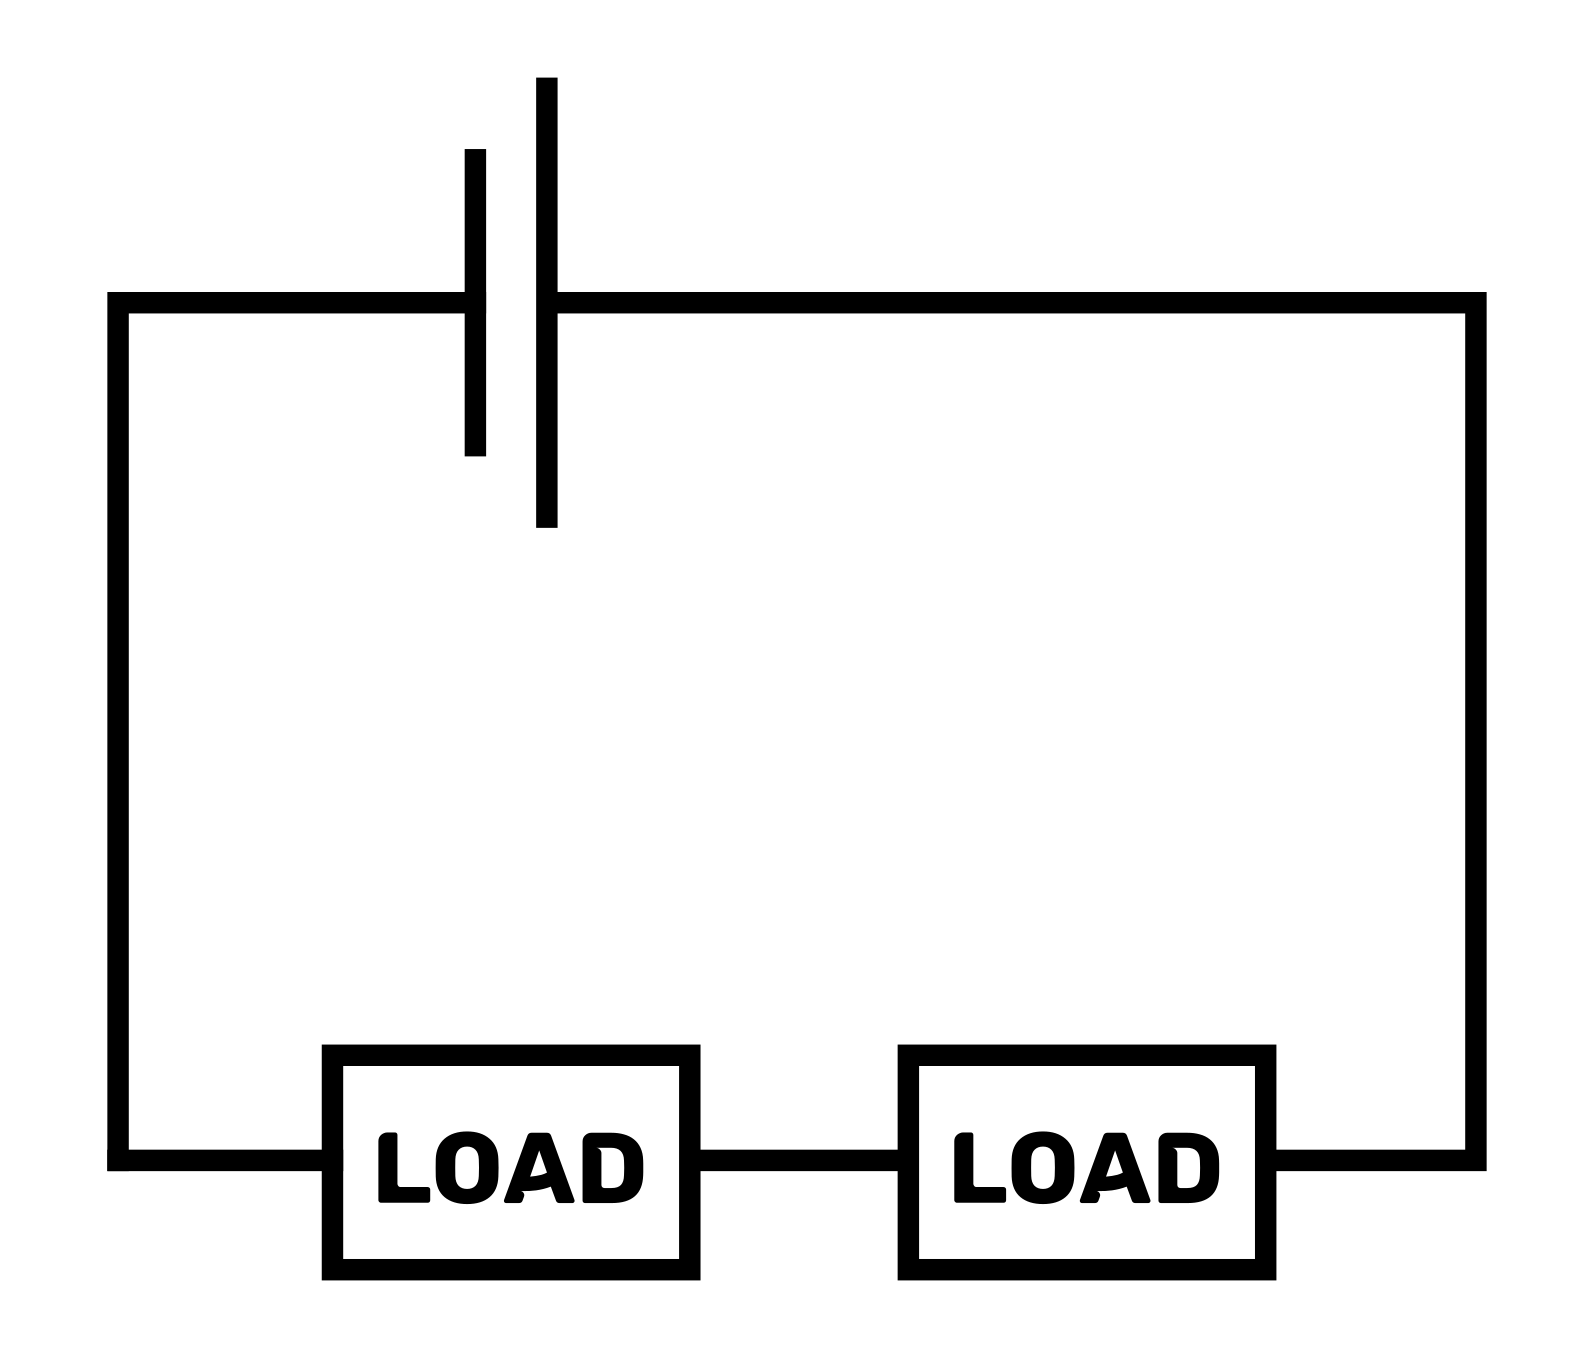
\includegraphics[width=0.5\textwidth]{series1}

A parallel circuit, on the other hand, has an equal voltage across each path, with the current being split. Because of this, resistors in parallel path will represent a resistance, lower than the lowest resistance of a path.

There is the below equation that can be used to calculate it-

\[\frac{1}{R_{total}} = \frac{1}{R_1} + \frac{1}{R_2} + \frac{1}{R_3} + \cdots\]

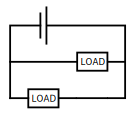
\includegraphics[width=0.5\textwidth]{parallel1}

Therefore, an example with the following circuit with 2 resistors of 3ohm and 7ohm, in parallel with a single resistor of 15ohm. You first add the series resistors, therefore $R_1$ can be represented as 10ohm and $R_2$ as 15ohm. Therefore, putting it into the equation gives us the below-

\[\frac{1}{R_{total}} = \frac{1}{10} + \frac{1}{15}\]

\[\frac{1}{R_{total}} = \frac{1}{6}\]

\[R_{total} = 6\ohm\]

\subsection{AC vs DC}

AC stands for alternating current, whereas DC stands for direct current. If you consider there to be two sides to a graph, with the direction of flow, and magnitude of voltage, DC can be seen to have a constant magnitude and direction of flow, compared to a sinusoidal voltage magnitude, causing the flow of current to vary in direction. It is typically given as an RMS voltage and a frequency. The frequency is the number of full periods that happen per second, typically given in Hz, where the voltage is an average value, taking the root mean square, which represents the DC voltage that has the same power/ heating effect. This is commonly seen with power from the grid, with voltages typically being 230V RMS, with a frequency of 50Hz in the UK.

\includegraphics[width=0.5\textwidth]{acsource1}\includegraphics[width=0.5\textwidth]{dcsource1}

\includegraphics[width=0.5\textwidth]{acwave}\includegraphics[width=0.5\textwidth]{dcwave}

Digital electronics is all done within the DC realm, but many devices still require AC. It is the standard for energy generation, and is how power is sent across the grid and to our homes. It is widely used for motors, and where large voltage transformations are required, such as microwaves. Semiconductor electronics primarily work within DC.

The course will touch upon ways to convert between AC-DC and the benefits of each for different applications.

\subsection{Resistors}

\Theory{What are Resistors?}

Resistors are one of the first key components to look at, which only require an understanding of the equations already discussed.

Resistors are components which are rated to have a specific resistance. Therefore, depending on the circuit, there will be varying levels of losses seen from them (depending upon both the voltage and current). They can be quite important components to use when a part needs a specific voltage close to that of the source/ input, or as a way of limiting current flow.

This is an illustration of both the main representations of resistors.

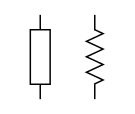
\includegraphics[width=0.5\textwidth]{resistor1}

This is a basic circuit, with wires, a resistor and a battery, to demonstrate V=IR. \href{https://tinyurl.com/27gj49kj}{Link}

In the specific example, we have a resistor of 1 Ohms and a voltage of 5V. Therefore, using $V=IR$, we can rearrange to find a current of $I = 5/1 = 5A$. This will find a power of $P = IV = 5*5 = 25W$. Each of these discussed can be seen in the simulation. Feel free to play around with it and alter values. Instructions in use of the simulation program can be found (here).

\Examples{Example circuits etc}

As this is early on, there aren’t too many example circuits just using the above knowledge alone. One example, would be if a project required use of a heater. Given that you know the input voltage that you have available, and the required thermal load, you can calculate the resistance of the heating element you require.

\subsection{Potentiometers}

A form of resistor is a potentiometer, which is a type of variable resistor acting as a potential divider, which uses a mechanical dial to alter the resistance at the output. There are a range of cases where this is helpful, such as altering the gain/ volume of a circuit or speaker, or where you aren’t certain on what voltage would be best. These typically have 3 pins, one for power/ input, one for ground and the last for the output, which with the input acts as a resistor of a voltage depending on how much the “dial” is twisted.

There are also digital Potentiometers, which are an example of an integrated circuit (see here), which can be programmed to act as a set resistance, using with set steps, so the same resolution isn’t usually attainable.

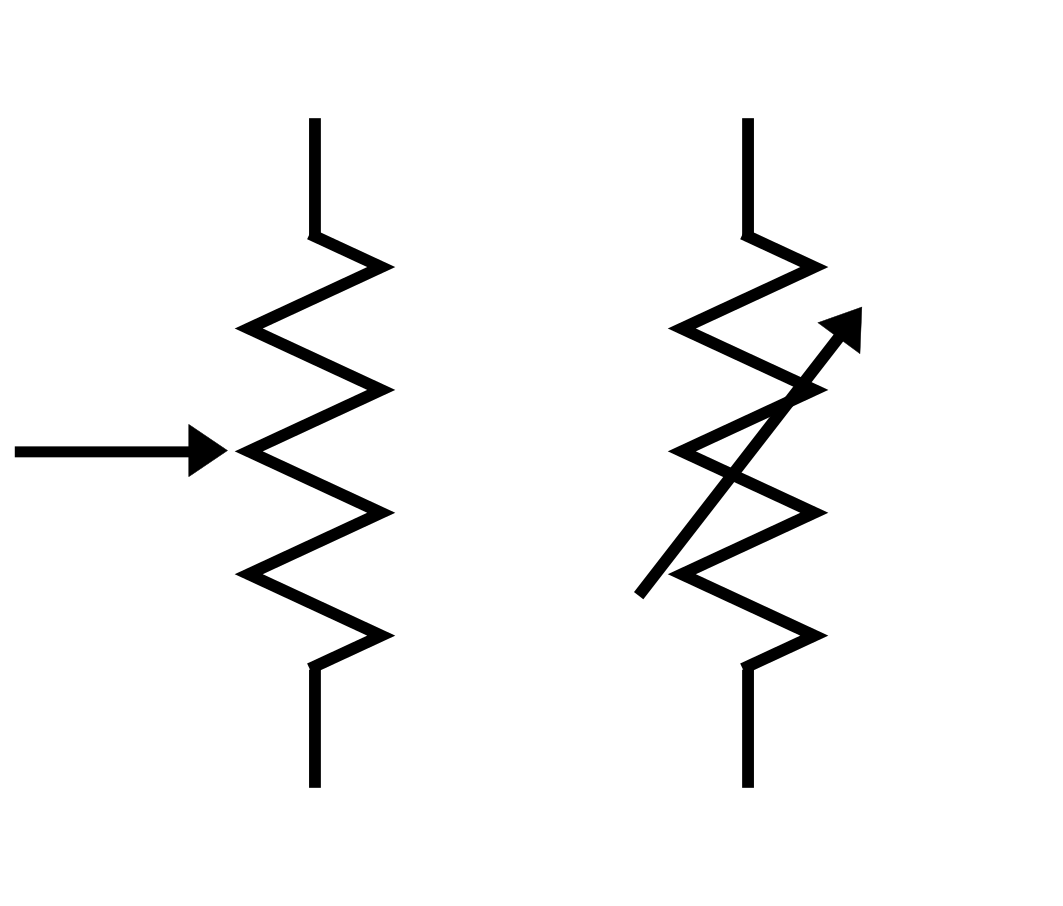
\includegraphics[width=0.5\textwidth]{potentiometer1}

\subsection{Capacitors}

\Theory{What are Capacitors?}

Capacitors are another key component key to electronics. They store energy as Electric Potential, with their voltage increasing towards the voltage of the input, as they are charged. Therefore, the charge and discharge curve is nonlinear, more following an exponential curve.

The unit for capacitance is Farad, with typical values depending on capacitor type, but usually in the uF units or below.

Capacitance can be related through a range of physics based equations, which will be touched upon now.

Due to capacitors being related to how its plates are charged relating to its voltage, there is the following basic equation- $q = CV$, where q is charge, C is capacitance and V is voltage. There is also the energy formula for calculating the energy stored within a capacitor, with the following basic equation- $E = 1/2*C*V^2$, where E is energy in Joules.

A resistor is usually placed in series with a capacitor to limit the inlet current provided to the capacitor. As it charges, the ratio between its voltage and the supplies voltage decreases, and as does the charge current, in a curve in the reverse direction to the voltage.

One of the built in simulation circuits from Falstad is helpful for showcasing the charge and discharge characteristics of a capacitor, by flicking the switch. \href{https://tinyurl.com/2erbz4jy}{Link}

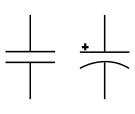
\includegraphics[width=0.5\textwidth]{capacitor1}

\Examples{Example circuits etc}

\Quiz{Quiz}

1. How do capacitors store energy?

a) In the magnetic field

b) In the electric field

c) As thermal energy

d) They do not store energy

2. True or false, a resistor is typically used in series with a capacitor to limit current flow through the capacitor.

3. True or false, 1 Farad capacitors are commonly available.

4. Design a circuit for charging a capacitor at a maximum current of 1A, assuming a source voltage of 3V.

\subsection{Inductors}

\Theory{What are Inductors?}

Inductors are the other main passive energy storage component. These store energy within the magnetic field, and have a range of uses, usually in power electronics.

The unit for inductance (L) is Henry, with typical values depending on inductor type, but usually in the uH or mH units or below.

Inductance can be shown through a range of physics based equations, which will be touched upon now.

There is the following basic equation- $L = \frac{\Phi(i)}{i}$. There is also the energy formula for calculating the energy stored within an inductor, with the following basic equation- $E = 1/2*L*I^2$.

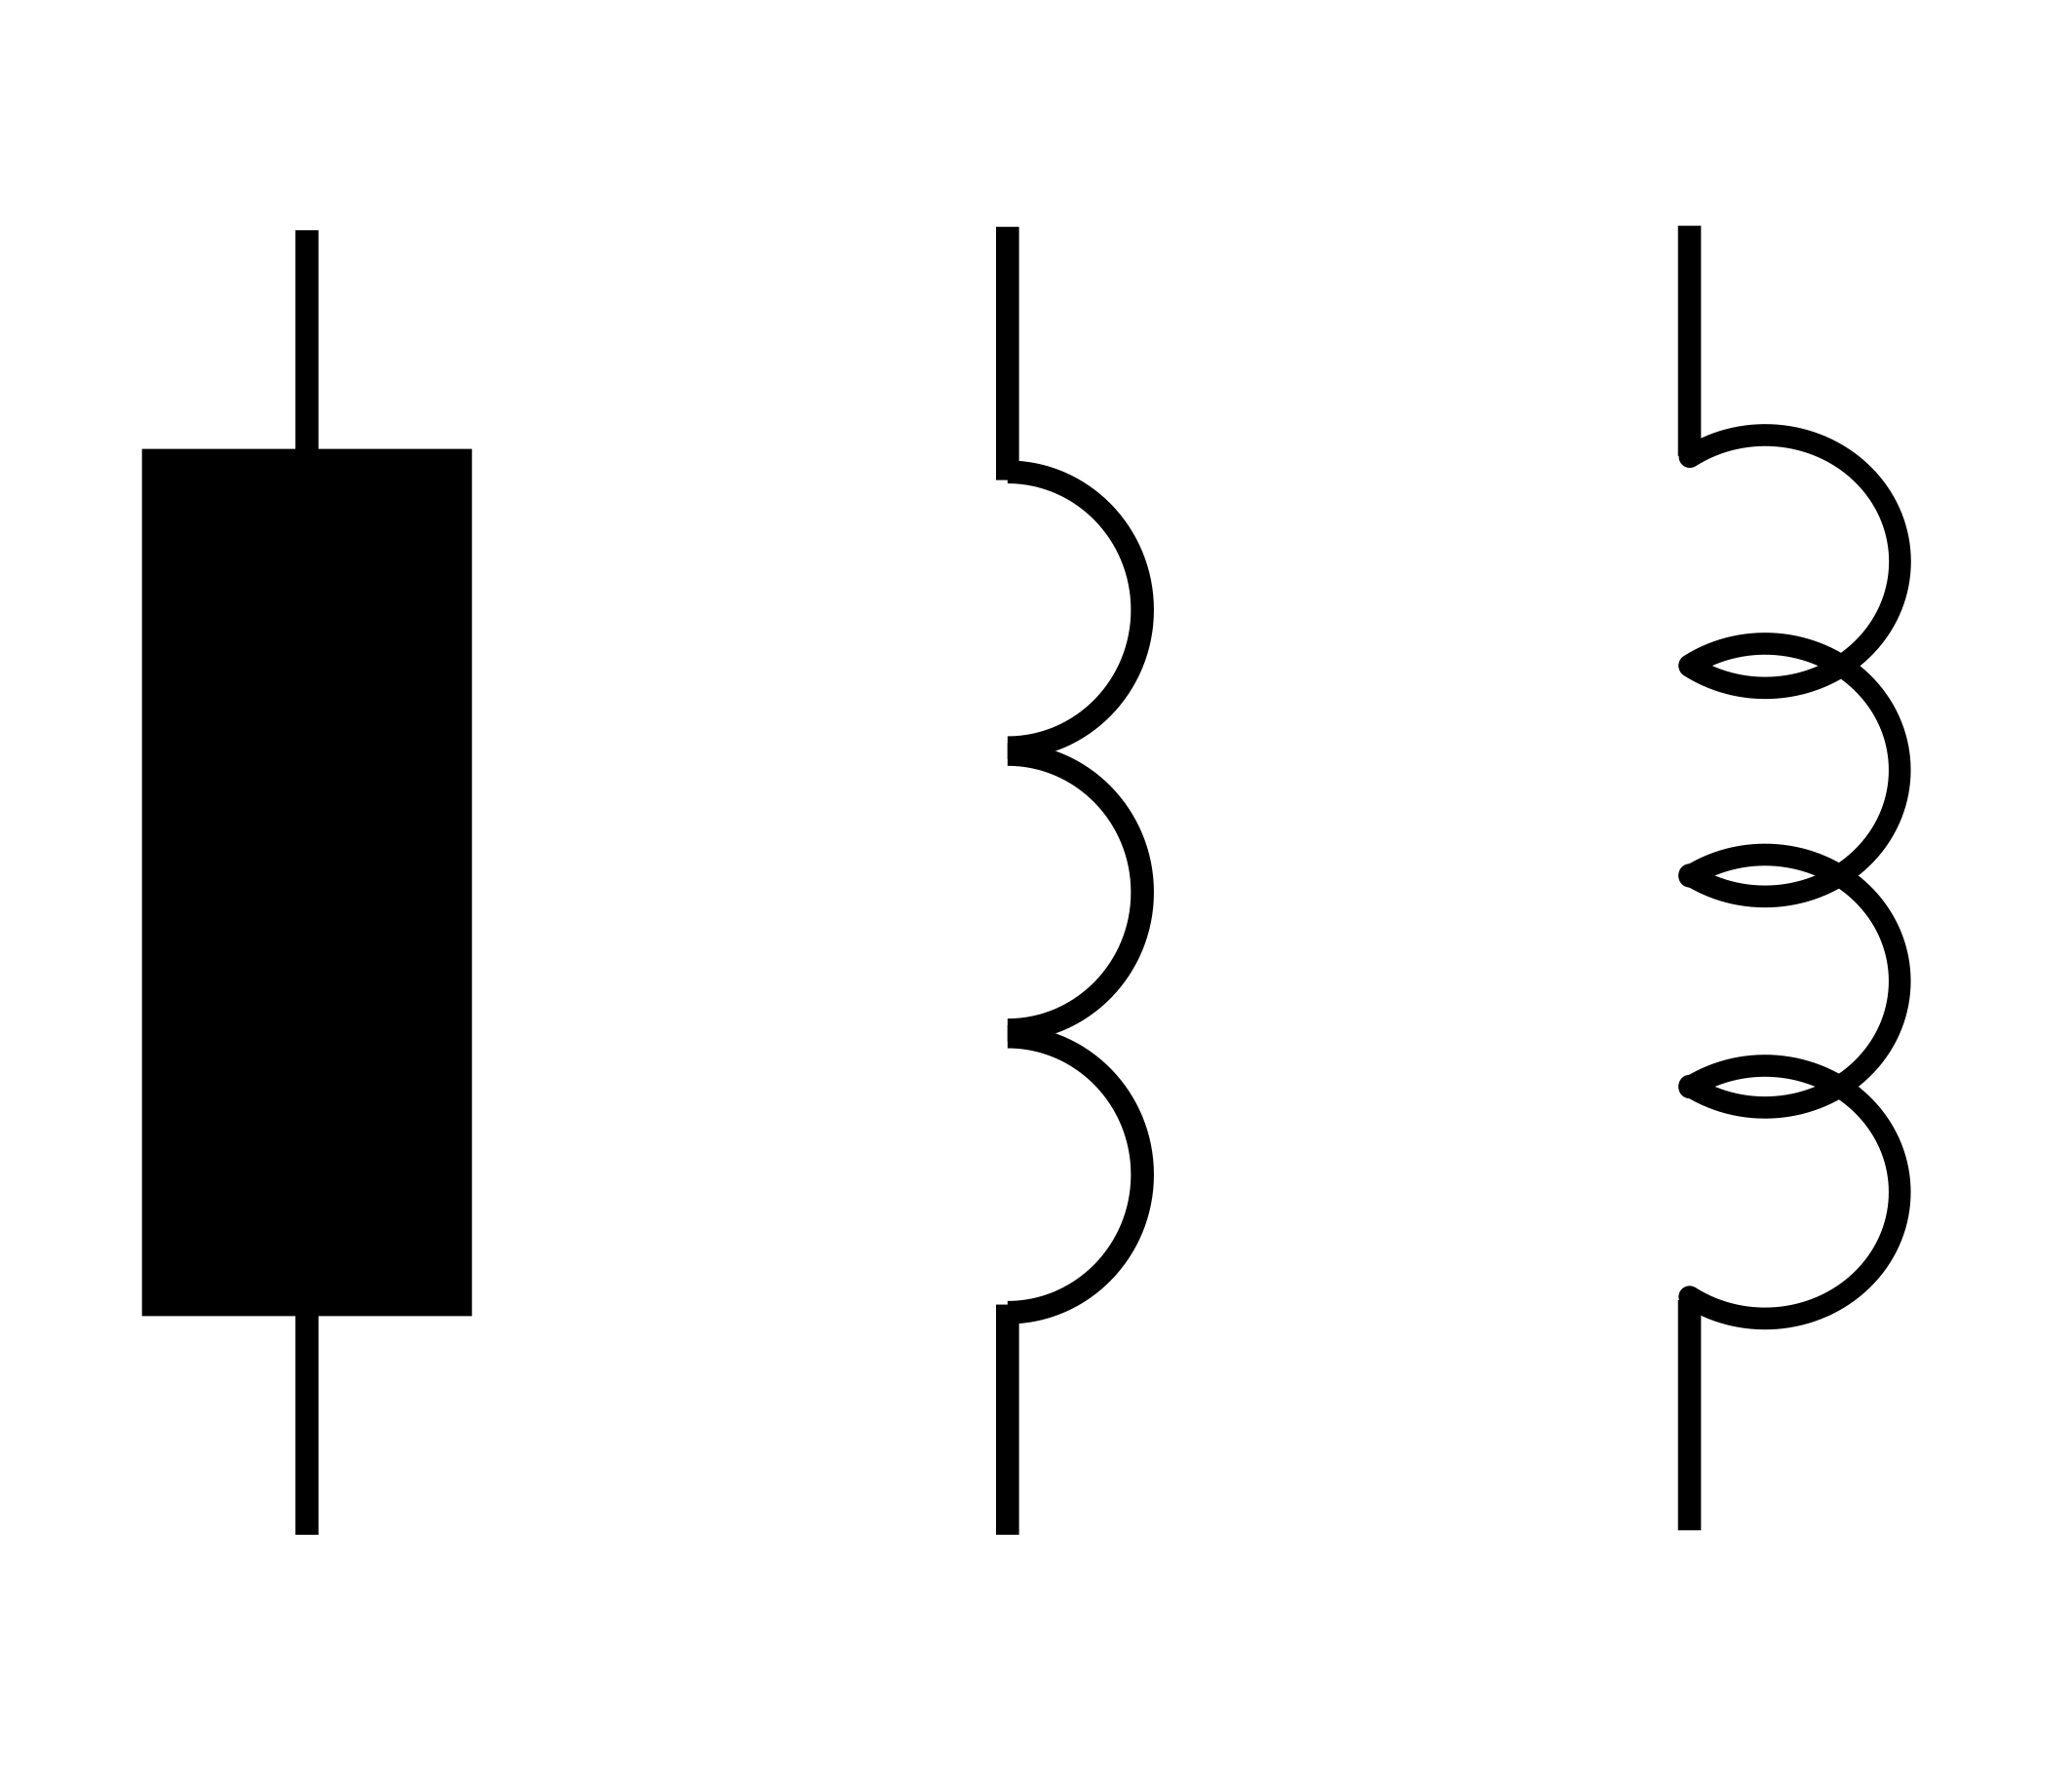
\includegraphics[width=0.5\textwidth]{inductor1}

\Examples{Example circuits etc}

\subsection{Analogue vs Digital}

It is important to be aware of analogue and digital and their differences. Analogue refers to a wave, so the fundamental characteristics which are altered are wavelength, frequency and magnitude. A key thing to be aware of is the fact that this magnitude can vary a lot and is a key reason for using analogue.

On the contrary, digital is represented with either 1 or 0, having an off or on region. As already touched upon, the entire field of digital electronics is based around semiconductors, which form switches.

Signals can be sent through both methods, with a range of benefits and negatives. A lot of data can be shown in a single analogue signal, although it's difficult to accurately read. Whereas, DC deals with two distinct boundaries, so although many more “pulses” are required to output the same amount of data, it is more reliable and easier to use/ read within logic based processing/ boolean algebra, which is touched upon later on in the course.

Sensors are often read using analogue methods, where there is an induced or dropped voltage which can vary in magnitude. This would need to be converted to a digital value for use within a circuit. A combination of digital 1/0 gives binary, which means a voltage value can be represented as a binary combination of 1s and 0s. As already touched upon, an ADC is an example of a component which can do this.

\subsection{Sensors}

\Theory{What are Sensors?}

Sensors are likely going to be one of the key components/ modules that you will use in your research, so understanding how they work and what options you have is important. There is a lot of sensors and sensor theory, so the key aspects will be discussed initially here, with more written in the further reading section, if you would like more depth.

This will be split into several sections, covering some of the major sensors, with more detail on sensors likely to be used within Chemistry related projects.

Sensors generally use resistance, capacitance or inductance to take a vast range of measurements, often using a MicroMechanical system (MEMS) to allow for this.

Temperature sensing can be done with a range of different methods, and is likely to be quite important. The most common sensors are analogue ones, where the components resistance changes along with a temperature change, although there are digital sensors for this too. There are four types of temperature sensor, which we will quickly touch upon each. There are Thermocouples, RTDs, Thermistors and specific digital ICs.

Thermistors are one of the more common types, and can be divided into NTC and PTC, with NTC being more common. NTCs have a decreasing resistance compared to temperature, and will have a resistance rating for 25C typically along with a value for how much their resistance changes per degree. Therefore, utilising a circuit to measure this resistance allows for a relatively accurate temperature to be read.

RTDs are similar in their operation to Thermistors, but are meant for a wide range of voltages, upwards of around 600C. Many comprise a length of thin wire wrapped around a ceramic or glass core.

A thermocouple comprises two differing conductors which generate a temperature dependant voltage. They have the highest temperature range of temperature sensors, upwards of around 1800C.

Digital temperature ICs will measure a temperature and report the data through transferring it through a specific protocol, which is discussed further (here).

Humidity sensors may be used along with temperature sensors, in a single digital package, or otherwise in an analogue form, where the humidity will alter the resistance of the humidity sensor. A couple of common digital examples include the DHT11, DHT22 and AM2320.

There is a range of sensors for detecting compounds in the air, particularly important to Atmospheric research. Usually these are doped so that an increase in concentration of a certain gas, such as carbon dioxide, would induce a voltage. Often because of the calibration involved and comparison with data, they can be quite complex integrated circuits, which will communicate via a protocol such as I2C or SPI to the microcontroller, later discussed in the protocols section. Although certain sensors may leave the conversion to the user. More modules are appearing in the market, which should help to ensure their accuracy, often key for taking useful measurements.

Photoresistors use a similar method but for light, where there is usually a resistance associated for them for pitch black, and a resistance for light, so an estimated light measurement can be attained from this. There are also photodiodes and photoresistors, each with their own benefits, such as a higher response rate to light, or costs.

There is a range of movement based sensors, which will quickly be touched upon. This will not be in great depths, as you are unlikely to require the use of these too much.

One of the main cheap and widely used range/ movement sensors is an Ultrasonic sensor, which has an ultrasonic transmitter and receiver, which using knowledge of the speed of sound, measures the time it takes for sound to hit a surface and reflect, to then calculate a distance value.

There are also LiDar sensors, which are similar but known to have higher precision, which use a singular beam of light, and calculate its time of travel, these are also known as Time of Flight (ToF) sensors.

The motion based sensors discussed above are ones that are contactless, but there are also contact based sensors, which a potentiometer could be an example of, using its resistance based on a linear or rotational movement as a measurement of movement.

\subsection{Diodes}

Diodes are widely used in electronics for a range of purposes. The basic principle of a diode can be thought of as a device/component which limits how current can flow within a circuit, such as restricting current flow to one direction.

This makes them beneficial for a range of circuits, such as protection circuits, preventing unwanted reverse current flow, which could damage other components or cause unwanted side effects.

They are one of the simplest examples of applications of semiconductors, where usually silicon is doped with other atoms to cause a surplus or shortage of electrons, changing the polarity of elements of the material, which is what effects how current can flow through the diode.

There are also Light Emitting Diodes (LEDs), which work through the same principles, but emit light of a set or alternating spectra depending upon selection. There is a voltage drop associated with this, but with considerably lower heat output, compared to filament bulbs, which worked by heating a filament to the point at which it begins to glow.

There is a common formula for calculating the resistor needed for an LED, given you know the voltage and current it runs at. This is the following-

\[R = \frac{V_s - V_f}{I_f}\]

Where $V_s$ is the supply voltage, $V_f$ is the forward voltage (voltage drop of the LED) and $I_f$ is the forward current.

Different colour of LEDs have different specific voltages that they work at, so this is an area where resistors are commonly used, to limit the current through the LEDs, while dropping the supply voltage to a voltage suited for a given LED. This voltage usually varies between around 1.8-3.3v, and is because of differences in how the semiconductor is doped, as it is the doping of other atoms which causes different wavelengths of light to be emitted.

It is important to consider that diodes have an inherent voltage drop, so this needs to be considered, especially when using them with low-voltage circuits, as a typical diode can have voltage drops between around 0.4-0.7v.

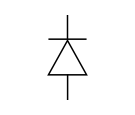
\includegraphics[width=0.5\textwidth]{diode1}

\subsection{Mechanical switches}

Switches are widely used as an input device, where depending if they are open or closed, can allow for power to be transmitted or not, by opening or closing a circuit. These can be split into many types, such as those which are usually open unless pressed, those which are usually closed unless pressed, those which switch between open and closed when pressed, and switches which you can switch to close several sets of pins/ connections.

This section will quickly talk through a few different switches/ buttons, their names and uses.

There are different switches that fit into different classifications, which will briefly be discussed.

Single Pole Single Throw (SPST) switches are ones which connect or break a connection between two single wires/ points/ terminals.

Single Pole Double Throw has a single input but two outputs which can be switched between.

There is then also Double Pole Single Throw, which is a combination of two SPSTs and Double Pole Double Throw, a combination of two SPDTs.

Now onto the different types of switch. They can mainly be split into several types, being the below-

Push button- A typical button, some of which will stay closed/ pressed until pressed again, when others such as momentary push switches will only be closed as they are pressed.

Slide switches can be flicked into a set position, and can be just between two positions or multiple.

Toggle is a slight adaptation of slide switches, flicking a centred switch from one angle to another, but otherwise it works through very similar means.

Rotary switches can twist to connect a pin with a range of other pins depending where it is twisted to.

You may have a range of switches, such as a few slide switches packaged together in DIP format.

\subsection{Digital switches}

Switches are widely used within electronics and are what has led to the field of digital electronics. Microcontrollers may use millions of switches on a single silicon die, where discrete switches tend to be used for power electronics.

Switches are important to have control of a circuit. These will be discussed in greater depth later on, but they usually have a gate which is triggered externally, which closes a circuit. So you can think of a switch as a tap allowing or restricting water to flow. The vast majority of these are semiconductor based, due to the low losses involved, although they are limited to DC function.

This document will quickly talk over the main types in some detail, so you can understand why each may be used, or why the surrounding circuit looks like it does.

There are current controlled switches and voltage controlled. BJTs are an example of a current controlled switch, where a flow between the gate pin and the emitter allows for a higher current to flow between the emitter to the collector. There is a voltage drop though, which can mean losses are fairly significant at lower voltages. They have the benefit of being quite easy to use in a circuit, after calculation of values.

Then there are voltage controlled switches, the main example of this being MOSFETs. These have a gate which is allow current to flow after the voltage is higher than a threshold value. They are more complex to use, since the gate acts as a capacitor, so has to be charged, so may not function well without a properly considered gate charge circuit. Losses are related to the MOSFETs internal resistance though, which can get very low, so they are typically fairly efficient.

There are other types, but these tend to be for power electronics, so we do not need to go into that level of depth.

Relays are an alternate form of switch, which use an electromagnet to cause a switch to open or close. These are particularly useful for AC applications, as most switches are limited to working with DC. They are another form of switch that provides electrical isolation between parts, as it is an electromagnet which pushes the switch closed.

Darlington transistors are also commonly known as a Darlington Pair, made of a couple BJT transistors, allowing higher levels of current amplification/ high current gain.

You can get arrays of transistors, such as Darlington Arrays, which is a chip with multiple Darlington transistors with common emitters. These are particularly useful for high power or inductive loads being controlled by a microcontroller.

\subsection{Opto-isolators}

Opto-isolators, otherwise known as optocouplers, are components that use light to transfer electrical signals between two isolated circuits. This is important if the two circuits run at differing voltages, or need to stay isolated.

They work through the use of an LED and a photo-sensor/ photo-transistor, so it is light that transmits the data, to keep them electrically isolated. They are useful for measuring AC using DC electronics, so have uses within AC-DC power conversion/ supplies.

It may be worth reading the sections on photo-sensors/ photo-transistors within sensors, as well as transistors and diodes to fully understand this.

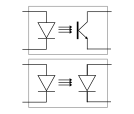
\includegraphics[width=0.5\textwidth]{optoisolator1}

\subsection{Ideal vs Non-ideal/ real components}

Until now, we have talked about components as if they are ideal. This means that they have no losses other than expected, which is not the case. Components will have an internal resistance, capacitance and inductance, which is worth being aware of. For more low speed circuit design, the internal resistance is the main thing you need to be aware of. This includes the source, with certain batteries/ sources having quite a high internal resistance, which means at higher current draws, there can be a fairly significant voltage drop before it even gets to the rest of the circuit. Any one of these factors can have a significant effect upon a more high speed circuit, with capacitance and inductance altering over different frequencies.

\section{Communication Protocols}

\subsection{Wired Communication Protocols}

Communication protocols are important to interface with different devices and equipment, so a base understanding of some of the major ones would be important.

Communication protocols are a set of rules which devices follow to transfer information, allowing coherent data transfer at set speeds, depending on the usecase.

It will first be useful to distinguish between serial and parallel, since these are widely referenced regarding communication protocols.

Serial means that there is a single data line/ wire used for communication in a given direction, where parallel means that there are several data lines or wires with data travelling through. Therefore serial is typically an easier to use or implement method.

They can first of all be split into two main kinds, with inter system protocols being those used to have communication between devices, where intra system communication protocols are meant for between component communication.

Therefore you may have to use a combination of the two, depending on what is being done.

USB and UART are the main examples of inter system protocols, where SPI, I2C and CAN are some of the main intra system protocols. It is worth remembering that although these are some of the main protocols, it is not a definitive list, with more niche or proprietary protocols also being around which can often have specific benefits, or are just used to limit use of other companies chips for a given application.

Master and Slave are still fairly common terms used within communication protocols, so you need to be aware of the terms, although there is a shift to alternate terms such as controller and responder, although there is not yet a set standard. Other alternatives could be on the lines of primary and secondary, leader and follower and source and sink, although the latter of which already is widely used within electronics. Due to the negative connotations of master and slave, this course will go with the suggested terms of controller and responder.

USB is very widely used, and is how many devices are connected to computers. It is high speed, and quite simple to implement, although requires the use of specific drivers as well as a powerful controller. USB 1 and 2 have 4 pins, one for power, one for ground and two for data, with data being sent serially in each direction.

UART is physical circuitry for conversion between serial and parallel data, where two UARTs may communicate with each other, communicating in serial, meaning that only two wires/ data lines are necessary for communication between two devices.

RS232 is another protocol (Recommended standard 232), which is often used within telecommunications. In general, kit is often used for connecting devices such as data aquisition or modems, the prior of which likely to be particularly important. When RS232 was created, it allowed for “handshaking”, which is a method for each device to check that data is being transmitted correctly, although many devices no longer require the use of this. RS232 can directly connect to the serial port of a computer.

ModBus is a protocol which was created for communication for programmable logic controllers, often for industrial use. One of the reasons for its wide usage is that it has no royalties and is open.

SPI is a common communication method, which can have a single controller and many responders connected to it. SPI stands for Serial Peripheral Interface, with there being 4 mains lines used, two pins for data transfer, a pin for selecting which responder the controller is communicating with and a line used as a clock. Therefore, for each device/ responder that the controller wants to communicate with, a seperate select pin is required. It is a relatively fast communication protocol, but doesn’t scale the best due to needing a new GPIO pin for each new device.

I2C is a similar communication protocol, which is also synchronous like SPI, controlled with a clock from the controller. It only requires two wires for communication, the clock and the serial data line. It can communicate with many devices/ responders just with these two wires, but is limited in speed and has a combined line for transmitting and recieving data.

CAN stands for Controlled Area Network, and is a protocol meant for the transmission and reciept of data within a network of devices, especially for harsher environments. Due to this, it is mainly used in industrial and automotive environments, so may be used by certain equipment used. It is fast, secure and low cost, but is complex and automotive orientated.

Since not all devices will have protocols that can be used together, there are chips meant for conversion of protocols, typically seen as modules which may need to be used to interface between a device and the computer. As previously mentioned, USB often requires drivers to be installed, so you should be aware that you may need to download a driver for.

This section will quickly go over modules/ chips you may come across for communication with these different protocols.

USB to UART modules are very common, often having a USB port on one side and 4 pins on the other. These may use a range of chips and are likely to use TTL level which is transistor-transistor logic between the limits of 0 and VCC which is often either 3.3V or 5V. A supplier will mention whether it works at TTL voltages, or others such as RS-232, a standard meant for telecommunications.

\subsection{Wireless Communication Protocols}

Although we won’t go into too much detail, it is helpful to be aware of some wireless communication protocols and their benefits.

WiFi- This is a family of wireless protocols, meant for local area networking, and is one of the most widely used.

Bluetooth- Bluetooth is a short range communication, meant for communication between a fixed and mobile device. It has been through several iterations, with Bluetooth 5.0 having distances upwards of 400m, but it is typically below 10m.

ZigBee- This is meant for creating local area networks of devices, with communication range between 10-100m.

LoRa- This is a long range radio protocol meant for unlicenced radio bands, with ranges in the KM range being viable, depending on the landscape and antenna used.

GPRS- This is the protocol which is the mobile standard for 2G and 3G mobile networks.

\section{Integrated Circuits (ICs) and Microcontrollers}

Along with some of the more discrete components mentioned above, there are many integrated circuits, which are components with a circuit built in, for set functions. A complex example of this, which is widely used is Microcontrollers. Microcontrollers are low power processing units, with built in memory, that can be programmed to do a range of functions. These may typically be put together as a single complete unit, such as an Arduino board. An Arduino is a board with a microcontroller and array of passives/ discrete components, so that it can be programmed from a computer, and interface with basic electronics components.

Integrated circuits may do a wide range of things, such as amplification, timing, power conversion. These help to decrease the time, complexity, power consumption and often costs of a design by packaging all the discrete components necessary for its function. Usually a few passives or discrete components may be used alongside it, with references to which parts being mentioned in a parts datasheet.

This section will quickly talk through some of the more important integrated circuits and their uses.

Amplifiers- A range of chips meant for the amplification of signals, usually analog signals.

Circuit Protection- A range of components meant to protect other aspects of the circuit, such as digital fuses or ESD protection.

Timing- A range of chips to provide the timing for other chips.

Data Conversion- Chips used to convert one type of communication protocol to another, or for analog to digital conversion.

Display/ LED Drivers- Chips meant for the driving of displays or LEDs.

Interface ICs- Chips meant for communication over different protocols, or to interface with different parts/ devices.

Communication ICs- A range of ICs and modules for wireless communication, such as WiFi, Bluetooth, LoRa, ZigBee.

Logic ICs- Chips that work through low level boolean logic, for building logic based circuits.

Memory- Necessary for storing data.

Power Management- A range of chips for power management, whether this is active or linear power conversion, battery management, power monitoring or other driving chips.

Sensors- A range of chips for interfacing with analog sensing elements or combining both into a single package.

As already discussed, there are a range of protocols which microcontrollers may be able to communicate by. They also may contain a range of integrated circuits, to help interface it with different components, such as with an analogue sensor. In this example, an ADC tends to be used (these are often internal to a microcontroller but you can get ICs specifically for this role). An ADC is an analogue to digital converter, which will represent an analogue value as a given bit size, depending on its resolution. This can allow a voltage reading to be associated with a digital value, which can be converted to a specific unit within the program.

\section{Boolean Logic}

Boolean algebra is a branch of mathematical algebra, where variables are either true or false, and it is centred around three main operators “And”, “Or” and “Not”, and several sub-operators.

For this section, the practical elements will be done through DDSIM, another online simulator, developed by a Lecturer at the University. Although similar functionality can be done through Falstad circuit simulator, DDSIM is more streamlined and intuitive for digital/ boolean electronics. Feel free to see which you prefer for which task, as they are not completely different.

https://www-users.york.ac.uk/~dajp1/Temp/ddsim.html

(There is also DASIM, for analogue electronics, similar to Falstad, where it can be easier to draw up circuits, it isn’t quite as easy to visualise, https://www-users.york.ac.uk/~dajp1/Temp/dasim.html).

First of all we will describe what the different operations mean. Think of it being a comparison of usually two inputs, either being true or false, on or off, a voltage being present or not, or 1 or 0. Since true and false is the terminology used within boolean algebra, this is the main terminology which will be used here. Firstly there is “And”, which is when both inputs are true, the output will be true, any other combination will result in a false output. Then there is “Or”, which states that if either or both of the inputs are true, the output will be true. The last main type is “Not”, which only has a single input, where if the input is true, the output is false, and if the input is false, the output will be true. Within electronics/ circuitry, gates areused to allow this logic, so you have And gates, Or gates and Not gates. There are several more complex examples, such as NAnd, NOr which are a combination of an And followed by a Not and an Or followed by a Not. Another more complex example is an Exclusive Or (XOr), which has an output which is only true if only one of the inputs is true. It is useful to know that it is transistors within electronics that can make up these gates, and that a combination of NAnd gates can create any gate. This has become the normal, since NAnd gates are quite easy to produce from transistors.

In the examples, we have used A and B as the inputs and O as output.

\includegraphics[width=0.5\textwidth]{andgate1}

\includegraphics[width=0.5\textwidth]{orgate1}

\includegraphics[width=0.5\textwidth]{notgate1}

\includegraphics[width=0.5\textwidth]{xorgate1}

Boolean logic is what has lead to computing, as it is a combination of logical operations done with gates. There is a set of fairly standard circuits that people are usually challenged to make, and it is useful to try and make some of these to make sure that you understand boolean logic.

\section{Electronics test equipment}

There are a range of pieces of equipment that can aide you with electronics, which some may seem overwhelming at first. But understanding what they do, and why/ if they are needed are important!

\subsection{Multimeters}

A very common piece of equipment is a multimeter. These are used to measure current, voltage and resistance. When measuring current, the multimeter needs to be connected in series with what you are attempting to measure, where to measure voltage or resistance, you place the probes in series with the component or circuit segment you are looking to measure.

There are both analog and digital format multimeters, with the latter being the more common, and what we will focus upon on this course.

There are a range of functions on a multimeter which I will talk through now.

You can measure resistance, current, voltage and continuity on most, with some having the function to measure the hfe or current gain of a BJT transistor. Some may also be able to measure capacitance.

Depending on the multimeter, some will split each of the sections into specific scales, representing the max value it can show. This is so the the resolution shown can be close to the scale of the measurement. If when trying to measure a value, nothing seems to be read, you may need to move this scale.

The continuity tester is used to check whether two points within a circuit are connected, or whether current can flow from one to the other, so can be very important for checking over soldering.

For most functions, connecting the cables to the V/\ohm/mA section would be suitable as well as COM/ ground, unless it is a high current circuit, if so there is the third connection usually for currents at a maximum of 5A or sometimes 10A.

A more complex piece of equipment which you may or may not use is an oscilloscope, which is again for measuring voltage and current, but comparing this against time, so graphs can be viewed/ produced using them. The software sometimes used within this course Falstad, uses scopes, which are a representation of what you would view through an oscilloscope probing a specific component or element of the circuit. It can be particularly helpful to check if the circuit is working as intended, or as an easier way to troubleshoot.

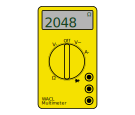
\includegraphics[width=0.5\textwidth]{multimeter1}

\subsection{Breadboards}

For electronics prototyping, breadboards are seen to be pretty important, as they allow you to connect up DIP components quickly for prototyping. They have many rows of 5 pins which are interconnected, so you can create an array of complex circuits with them, to quickly test out ideas. It is important to consider that they may not produce the most stable of circuits, and would not be recommended for the field due to loose connections.

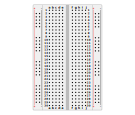
\includegraphics[width=0.5\textwidth]{breadboard}

Internally, it is just rows of interlinked metal, which connect/ bridge pins together. As can be seen, there are two sets of 30 rows of 5 pins, with each pin on that row connecting, so two parts that need connecting, should be connected to the same row. There are also power rails, which allow for 2 different voltages, and two sets of ground pins. These are there for convenience, rather than being the only suitable sections for providing power, so if necessary, a row of pins could be used for other voltages. Breadboards are specifically meant for DIP components, with the gap in the centre allowing for DIP chips to be placed, seperating each of their pins. Components can be connected with male to male jumper wires. As mentioned, it is worth only attaching power when you are sure that everything is firmly connected, with no potential for shorts. There are limits to the suitability of a breadboard circuit, it is meant for lower power and lower speed circuitry.

\Examples{Examples}

Here are a range of example circuits, to help you to understand how a breadboard circuit should be wired, with increasing complexity.

The first example would be an LED with resistor, a button and a battery.

\Quiz{Challenges}

1. Connect up a circuit with a blue 5mm led, 2 AA batteries, a 50 ohm resistor and a momentary push button.

2. Connect a circuit with 2 AA batteries, with a blue LED, resistor and button, in parallel with a red LED, resistor and button. You will need to calculate the resistor required.

It would be good to have the ability to build a breadboard circuit, so here are a range of challenges. You may need to read other sections of this course if you are struggling.

The next stage from here is either a protoboard design, such as using vero or strip board, or the design of a custom circuit board, or use of existing modules suitable for the design. The cost of custom printed circuit boards have come down considerably over the past few years, through sites such as JLCPCB, so it has now become more of a viable option for designs for use in the field.

In the further reading section, there may be small amounts of detail on PCB design or resources helpful for doing this, but it is not the focus of this course.

\section{555 timer}

555 timers are fairly adaptable circuits, for a range of timing technqiues, that may not require a whole microcontroller. Although understanding the internal structure of a 555 timer is out of the scope of this course, understanding how and why they are used could be beneficial.

Depending on how it is connected to, it can be used for outputting waveforms of different frequencies, or as a timer.

\section{Amplifiers}

Amplifiers are there to increase the amplitude of an analogue signal, often useful for use alongside analogue sensors, to take it to a voltage range readable by a microcontroller. A common component for amplification is an OpAmp, which can be wired in a range of ways, such as through amplifying a voltage difference, or amplifying a signal by a specific amount in either the positive or negative direction.

Again, an understanding of how amplifiers work internally is beyond the scope of this course, although understanding of what you can do with them is helpful. We will touch upon the types mentioned above in some further detail. Each of the below use an op-amp as the main component.

The main focus will be on use of opamps to create amplification circuits.

The first is not an amplifier, but is important to seperate two elements of a circuit. This is known as a voltage follower, which isolates the resistances at either end of the part, particularly important where you may be trying to read a resistance value from a sensor.

There are non-inverting and inverting amplifiers, which the first of which amplifies a voltage in its current direction/ magnitude, and the latter amplifies a voltage in the negative/ opposite direction or magnitude.

There are summing amplifiers which can be used to add two voltages together.

There are also differential amplifiers which will output the difference between two voltage inputs, with a certain level of amplification.

\section{Power conversion}

Power conversion could have a course on its own, so this will just lightly touch upon conversion, as a base understanding of it, and why it is important would be useful. Within the further reading section of this course, there is some information on Rectification, which combines knowledge learnt above, so is worth checking if you want more of a challenge, or need to know about AC-DC conversion.

The main types of power conversion are active and linear. Active utilises both capacitors and inductors, as well as switches for efficient conversion of voltage, either to a higher or lower level, with efficiencies into the 90\% possible. Whereas linear power conversion is cheaper, requires lower number of components and is specifically for decreasing the voltage at the output. It acts as a variable resistor, to dissipate the unwanted voltage as heat, so depending on the circuits needs, can be particularly inefficient. Therefore, if efficiency is less important than costs, or the voltage decrease is only very minimal, linear voltage converters can be an okay option. Given how easy it is to purchase a power conversion module (either known as step-up or step-down, whether the voltage is increased or decreased), in most cases this would be the best option, as all that is needed is to alter a potentiometer to get the output voltage you would like, with minimal losses.

To very quickly give the basics of how an active power converter works, a switch is turned on at a set ratio to charge and inductor, which then discharges to charge a capacitor, to give a smoothed voltage at the wanted level. The ratio between the switch on and off times will affect the output voltage.

The above mainly discussed DC to DC power conversion. To do AC to AC, a transformer is commonly used, AC to DC may use a similar method to above but using a transformer rather than an inductor, and the use of a rectifier to convert the AC to DC.

\section{Necessary software}

Throughout this document, you are encouraged to check simulations through Falstad. Falstad is a web-based, simple to use but relatively powerful circuit simulation program. It was designed orginially by Paul Falstad and is completely free to use.

It has been selected due to its ease of use, and ability to represent information about the circuit in a clear and helpful way.

This can be found through the following link- \href{https://falstad.com/circuit/}{Link}

It provides a visual and easy way to represent circuits, with the ability to plot voltage vs current for set positions or components. There is a vast array of sample circuits which can be looked at for reference too. The simulations mentioned in this course use this software, so a brief understanding of how it works would be useful. Each component will have nodes/ squares where other components should be connected to. These components can be found in the draw section, and you can click and drag to alter its size.

LabVIEW will be required for the practical element of this course. LabVIEW is a graphical programming plaform, specifically intended for Test and Measurement, so was selected as a suitable program for testing out the skills developed through this course. This will need to be installed, using the Universities licence, which the steps can be found through the following resource- \href{https://www.york.ac.uk/it-services/software/a-z/labview/#tab-2}{Link}

LabVIEW will be used to interface with an Arduino, rather than using a programming environment such as the Arduino IDE. It is useful to quickly mention though that platforms such as this are often used to program microcontrollers such as an Arduino, which uses C++, plus some specific methods/ functions.

\section{Electronics safety}

Safety is something that is a key consideration when doing anything with electronics. If you are unsure, it is always best to ask rather than to assume.

As has been discussed beforehand, current can be related to voltage and resistance through $V=IR$. The body has a resistance which can vary depending on length etc, but is relatively high. Therefore, as voltage increases, so will current if the resistance stays the same. It is always good practice to take caution when using electronics, but especially when dealing with higher voltages, as it can be fatal. It is likely that the voltages used for the in-person practical elements will be low voltages. It is important to know when you are not confident or don’t know the risks with a given piece of electronics and know when it might be the better option to have someone else repair something. It is important to also consider that sometimes the best option is to replace something rather than make a repair, which could potentially be dangerous, or end up costing you more if it isn’t reliable, or takes a considerable amount of time to fix.

Something that might not be initially considered is ratings of components. This is something that is very important, to ensure that a selected part can take the expected power loss without damage. Therefore it is important when selecting a resistor to calculate its estimated power drop, and select a resistor with a power rating clearly above the max predicted power losses. It is important to add a safety buffer, as circuits in reality are not ideal, so may react slightly different than expected, such as a component having a resistance value that differers from its value.

Regarding differing values, a tolerence can be found, which is the percentage at which a value can differ. This is usually under 20\% (it can be considerably smaller). If you are unsure, it is better though to add a safety buffer, x2 the calculated value is fairly common, as it helps to account for how the tolerences of other components affect that one.

It is important to consider that all components have losses, including wire, so this needs to be considered, with a wire or connector of suitable ratings selected. With this waste heat, also comes a voltage drop, which may also be a factor, as if high enough, can cause issues with the circuit itself.

For wires, you have different wire gauges, and sometimes different materials. Typically wires will be copper, but sometimes they could be aluminium, which has a resistance around 64\% higher than copper, so looking at wire gauge alone isn’t always enough. Again it is helpful to keep the chosen wire a fair bit above the power rating you require, considering that only just meeting those ratings will lead to considerable losses in the wire. And if there are cost constraints, it is important to consider that a thinner wire which is initially cheaper may end up costing more due to electrical losses.

There are a range of types of connectors too, depending on the application, each of which that have their own rating. Mechanically connected, such as screw terminals are likely to have a resistance higher than directly soldered, but can give more flexibility to make alterations.

You should be careful when handeling components, as built up static can cause damage. Grounding yourself, such as touching a metal surface can help to reduce this static potential. Anti-static wrist straps are something that can be sourced cheaply to limit the potential of causing damage.

Soldering may be something that is required for a project. There are health risks associated with all forms of soldering, so it is best to solder in a well ventilated area with the suitable equipment. If possible, although slightly harder to work with, it would be recommended to use lead free solder, reducing health risks and allowing for safer use in the field. Within solder, there is flux which helps solder to flow better, but the evaporation of this produces a vapour which can be harmful if inhaled. Many soldering iron setups have extraction next to the iron, to minimize this chance of inhaling it.

Before connecting wires, particularly at higher voltage levels, running your hand along a cable to check for potential damage is important, replacing a cable if this is the case. It is also good practice to ensure both sides of equipment being connected are turned off before and during wiring, to prevent potential sparks, damage or electric shock.

Certain components can still be dangerous whether or not they are powered, a good example of this is capacitors, which can still hold power after the circuit has been turned off. Therefore, you should ensure not to touch one/ short it. It is good practice to have bleeder/ discharge resistors connected at either end of high voltage capacitors so that when not powered, over time they will discharge. This will add some inefficiencies to a system, but improves safety.

As has already been mentioned, it is important to ensure components are not shorted, as this can cause damage very quickly as the source will pump as much current as it can into the circuit, causing very quick heat up. Storage of components such as batteries in a proper case is important to ensure that they cannot get shorted. Ensuring to check over soldered circuits to make sure nothing is bridged, such as through use of a combination of a microscope/ magnifier, and the use of a multimeters continuity checker, as mentioned previously.

\subsection{Soldering}

As has already been mentioned above, being able to solder is an important skill to have. Usually someone would first make a circuit using DIP components before attempting more challenging SMD components.

Soldering is the process of creating a metal joint between a component and a circuit board, to allow for a considerably improved electrical, mechanical and thermal connection. Solder is typically in wire form, but can also be in paste form, and it is a metal with a low melting point, allowing for a quick connection to be made with a reduced risk of damaging components.

The most basic form of soldering uses a soldering iron, and solder wire. It is recommended to use a holder, which can hold the parts in place, to free up hands for soldering. The soldering iron should be placed so it heats up the metal of the component as well as the interface metal, with solder wire placed at the other side so that the solder can bridge the two, making a clean connection. A clean connection should be made if there looks to be a clean flow between the two parts, rather than a ball of solder or similar.

Sometimes too much solder may be added, and there can be some difficulty in removing this. A solder sucker can help, where you remelt the area with excess solder and then quickly press the solder sucker just above, which uses suction to pull up the excess solder. Solder wick is another option, which I do personally prefer, as you place it between the excess solder and your soldering iron, where it “wicks” up the additional solder. Keep in mind that this tends to be copper, so heat will pass through it very quickly, so keep hands far enough from the interface point.

Soldering temperature is important, it is worth looking at the melting point of the solder you are using, with lead free solder typically having a slightly higher melting temperature of around 217C, depending on composition.

Although lead free solder is known to be slightly more difficult to use, being better for the environment and for your health for me definitely makes it the better option. I haven’t found too much of a difference in using each, especially if a good quality soldering iron and solder is used. Also learning the easier option, which is only really suitable for DIY projects, and one which may get phased out in the not too long future, wouldn’t be the best idea.

\section{Component footprints}

It is important to be aware of the fact that components can be sourced in a range of footprints, which may be necessary to look into for electronics design or repair. Imperial measurement is most commonly used for surface mount resistors, capacitors and inductors, with values associated with mils, which represent 1000th of an inch. In many cases surface mount components will be used with commercial products, so use of one may be required in replacement of a faulty part. Understanding their size, and your ability to solder them is important, and it is often a challenge that people follow to trial their ability. You may be able to access a soldering oven, which can help make this process easier, considering that as solder melts, it can somewhat help to pull a component into place, if it is minorly offcentered.

It is important to consider that components are only rated to take a certain amount of heat, so care should be taken to not break components through thermal damage. If a component with multiple pads are being done, there could be time between the pins to allow a cooling period, to prevent large heat build up which has the potential to do damage.

\section{Further reading}

This section is here to provide some further reading into more advance topics. Although you may not need to make a circuit using the below, understanding of them may come in beneficial. Some of the below circuits also will help to solidify your understanding of the key components mentioned above.

\subsection{Rectification}

\Theory{What is Rectification?}

Rectification is the process of converting AC to DC, commonly used in power supplies, such as a phone or laptop charger. This is very important due to digital electronics requiring DC to function. Although repair/ diagnosis of AC circuitry should not be undertaken without the necessary training, understanding of how AC circuits function is important for safety and to better understand the use of different components.

\textit{This circuit uses components which have already been discussed earlier in this document, so for further explanation refer back to the appropriate sections.}

For this AC-DC conversion, the alternating current needs to be converted to flow in just one direction. Therefore a key component in this process is a diode (This will provide a hyperlink to the diode section).

The most basic form of circuitry is a half-bridge (otherwise known as half-wave) rectifier. This uses a single diode in series with the load, to only allow current flow in one path. Therefore, the output wave will be only the positive side of the sinusiodal wave, meaning that the average voltage seen at the output would be around half of the RMS voltage, although in a form likely unsuitable for most DC circuits.

\vspace*{1\baselineskip}

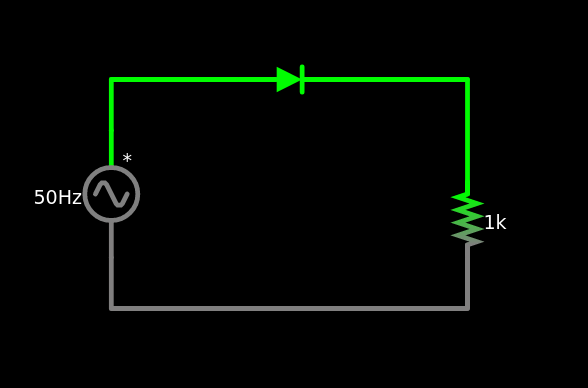
\includegraphics[width=0.5\textwidth]{halfbridge}

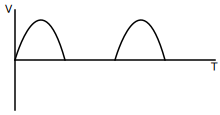
\includegraphics[width=0.5\textwidth]{halfbridgewave}

\vspace*{1\baselineskip}

A half-bridge circuit can be improved through use of filtering, with the addition of a capacitor to smooth the output voltage. This capacitor is added in parallel, where it is charged by the voltage, which it will then output this when the output drops below its own voltage. This means that the output voltage can get closer to being a smooth DC voltage. As previously mentioned, even if perfectly smoothed, the max voltage that could be attained is half the RMS voltage.

\vspace*{1\baselineskip}

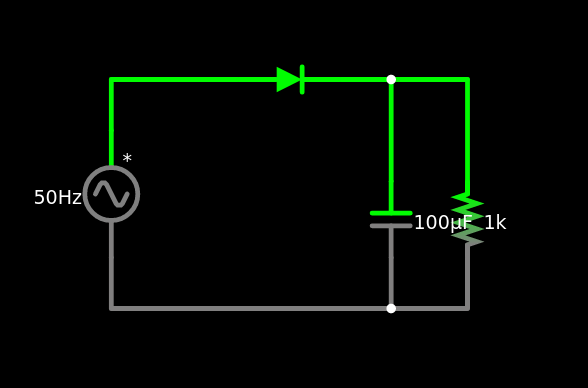
\includegraphics[width=0.5\textwidth]{halfbridgesmoothed}

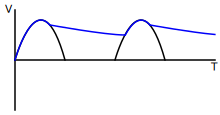
\includegraphics[width=0.5\textwidth]{halfbridgewavesmoothed}

\vspace*{1\baselineskip}

The next step to improve a half-bridge circuit is to make it a full-bridge rectification circuit, which utilises four diodes, meaning that whichever way the current flows at the input of the rectifier, it will be fixed at the output. Therefore there will be a sinusiodal voltage magnitude but only in the positive axis. This can again be smoothed with a capacitor, and if perfectly smoothed, can have a fixed output closely following the RMS voltage.

\vspace*{1\baselineskip}

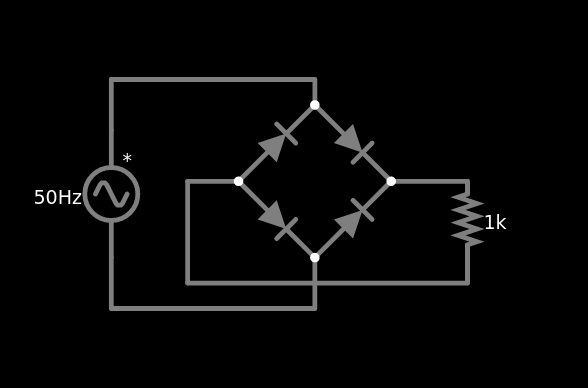
\includegraphics[width=0.5\textwidth]{fullbridge}

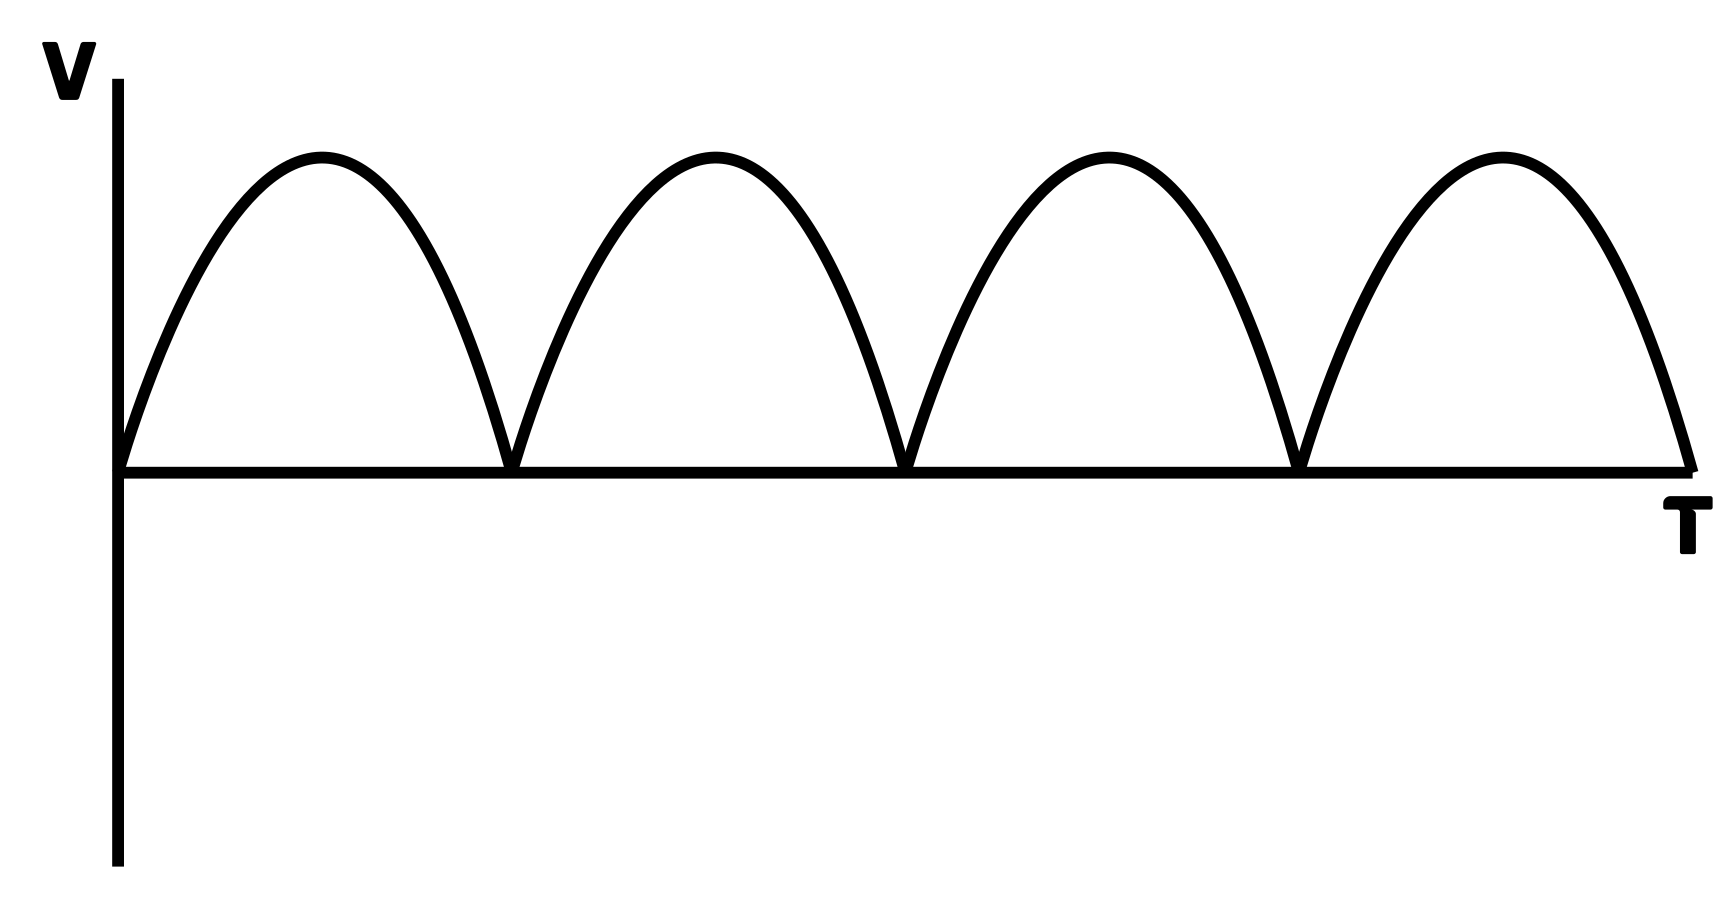
\includegraphics[width=0.5\textwidth]{fullbridgewave}

\vspace*{1\baselineskip}

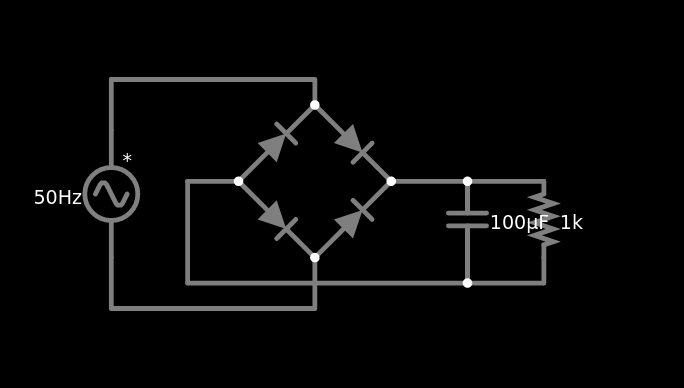
\includegraphics[width=0.5\textwidth]{fullbridgesmoothed}

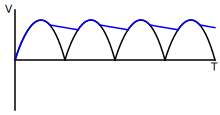
\includegraphics[width=0.5\textwidth]{fullbridgewavesmoothed}

\Examples{Example circuits, applications and considerations}

This section will quickly look at applications of the above mentioned circuits.

Rectification circuits are used a considerable amount, especially for AC-DC power supplies, as an initial stage to convert AC to DC. Due to this, their main usage is within power supplies connected to the mains. Other applications though could include a dynamo torch, where the AC power generated from the motor needs rectification to suitably power an LED.

It is likely that in the majority of cases a full-bridge rectifier would be used rather than a half-bridge rectifier, unless initial costs were a major consideration.

Due to varience in the manufacturing process, even within a single product, it is commonly considered best practice to use a full-bridge diode package, where there are four equal diodes within one part.

Rectifiers are generally used as part of a more complex power system, usually as an earlier on stage.

\Simulation{Simulations}

Below are several Simulations to have a play around with to help your understanding of Rectification.

Half-Bridge rectifier at 230V RMS, 50Hz- \href{https://tinyurl.com/24lw5qjj}{Link}

Half-Bridge rectifier at 230V RMS, 50hz with capacitive smoothing- \href{https://tinyurl.com/27lb3k8o}{Link}

Full-bridge rectifier at 230V RMS, 50Hz without smoothing- \href{https://tinyurl.com/224uqhfw}{Link}

Full-bridge rectifier at 230V RMS, 50Hz with capacitive smoothing- \href{https://tinyurl.com/2yeg4kof}{Link}

\Quiz{Quiz}

1. What is the main benefit of a full-bridge rectifier over a half-bridge rectifier.

a) It is cheaper to build.

b) It allows for full utilisation of the input voltage.

c) It uses less components.

2. Why are smoothing capacitors useful? (There may be more than one right answer)

a) They allow for a more constant output voltage.

b) They increase average power output.

c) They reduce output ripple.

3. True or False, it is known to be better to use several diodes individually rather than packaged together as a full bridge rectifier package.

4. True or False, rectifiers can be used to also convert DC to AC.

Challenge- Using Falstad or hand drawn, design a full-bridge rectifier with voltage variance/ ripple lower than 10\%, working with an AC voltage of a peak value of 326V, at 50Hz.

\pagebreak

\subsection{Gate Driving}

\Theory{What is Gate Driving?}

Gate driving is necessary for using MOSFETs in high speed circuits. Like mentioned earlier, MOSFET gates have an inherent capacitance which requires charging in order for the gate to “switch”. Therefore, for fast switching it may require large amounts of current, which a microcontroller may not be able to supply. Therefore there are integrated circuits with common methods to allow for these to be charged safely. One of the main simpler methods is called a totem pole gate driver. This uses a set of two BJT transistors, one which is used to charge and the other to discharge the gate. BJTs are used because of their simplicity, and ability to amplify the input current using an external source. Even then, it is important to use a resistor to limit the charge current for the gate.

This section has been written as it references a range of components and knowledge from the main sections of the course, so is a useful way to better understand theory.

Here is a circuit of it in action, feel free to play around with it- \href{https://tinyurl.com/2m77d6zl}{Link}

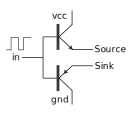
\includegraphics[width=0.5\textwidth]{gatedriver1}

\section{Resources}

There are many resources within electronics which can be helpful, both for learning more, but also for a range of different aspects. This will list some of the ones particularly worth looking into, and what they are for.

\subsection{Manufacturers}

It is useful to be aware of some of the main/ most reputable manufacturers of components as well as modules. This is certainly not a definitive list, but in mot cases you should be able to trust components from the below manufacturers. This will focus on some of the larger manufacturers, so there are many more trusted manufacturers. Keep in mind that there are fake components in the marketplace, so this is if you have sourced them from a trusted supplier, which is talked about in the section below! As touched upon in the finding components section, most parts through a site such as DigiKey should be trusted and reliable.

Resistors- Yageo, BOURNS, Panasonic, ROHM, Samsung, TE Connectivity, Vishay, Walsin.

Capacitors- Rubycon, Panasonic, Hitachi, Sanyo, Vishay, Nichicon, NCC, Wurth, Illinois Capacitor, Cornell Dubilier.

Inductors- Wurth, Walsin, Vishay, TDK, TE Connectivity, Pulse Elec, Murata Electronics, BOURNS, EATON.

Transistors- Vishay, TOSHIBA, Texas Instruments, STMicroelectronics, ROHM, RENESAS, onsemi, NXP Semicon, Nexperia, Infineon, Diodes Incorporated.

Diodes- Vishay, TOSHIBA, STMicroelectronics, ROHM, onsemi, Nexperia, Microchip Tech, Infineon, Diodes Incorporated.

Sensors- Infineon, Analog Devices, OMRON, Texas Instruments, TE Connectivity, NXP, Microchip Technology, Murata, BOSCH, STMicroelectronics.

Microcontrollers- Microchip, ATMEL/AVR, NXP, STMicroelectronics, Espressif Systems, Infineon, Altera, Raspberry Pi, RENESAS.

ICs- Texas Instruments

\subsection{Suppliers}

Starting with several trusted parts suppliers.

Arrow Electronics- Europe based Electronics components shop.

RS Components- UK Based Electrical and Industrial components shop.

Mouser- US based Electronics components shop.

Farnell/CPC- Electronics components shop based in several regions.

LCSC- Electronics components shop based in China, with links to JLCPCB and EasyEDA, offering lower costs than most other suppliers for larger orders.

Digi-Key

Rapid- UK Based Electrical and Industrial components shop.

EuroCircuits- Lower cost PCB manufacturer based in Europe.

JLCPCB- Low cost PCB manufacturer based in China

Aisler- Lower cost PCB manufacturer based in Europe.

The majority of the above focus on singular components, which may not be what you are looking for. If you are looking more for modules or DIY components, there are a range of other trusted retailers.

HobbyTronics- UK Based hobbyist electronics shop.

Bitsbox- UK Based hobbyist electronics shop.

Adafruit- US Based company producing a range of boards/ modules.

Sparkfun- US Based company producing a range of boards/ modules.

Pimoroni- UK Based module maker and hobbyist electronics shop.

As almost a subset of suppliers, there are a couple of sites used to find stock of certain components across suppliers, while comparing their costs. Within these tools, there can be a range of other suppliers mentioned, quite a few of these coming under the reseller categories, where you may be paying more, but they often have a range of parts other suppliers may not have.

These could be thought of Electronic Part Search Engines.

Octopart

Findchips

OEMSecrets

EasyBom

Electronics Software-

There are several bits of Electronics Software mentioned below, whether it is for simulation or PCB design.

Falstad- Free online electronics simulation program, which is easy to visualise what is happening in a given circuit.

LTSpice- Free and powerful electronics simulator, although slightly dated presentation, produced by LT.

TinkerCAD- Simple online software for basic 3D design and electronics design/ simulation.

MicroCap 12- Although it can be seen as abandonware, it is now free, relatively recent and a powerful piece of software.

KiCAD- Free and Open Source PCB Design Package

EasyEDA- Free and easy to use PCB Design Package with links to both LCSC and JLCPCB.

Another helpful resource could be additional places to go to learn further.

Allaboutelectronics

There are a range of helpful YouTube channels, such as the below-

GreatScott- Page with many tutorials and projects, in quite a lot of detail, although it can be quite complex for beginners. But if you like being taught through a project based idea, this is worth checking out.

Electronoobs- Another project based channel, teaching you a range of things.

EEVBlog- One of the biggest Electronics Video Blogs, covering a vast range of areas of knowledge at different levels, from an Electronics Engineer. Known to be unscripted, and “off-the-cuff”, but usually very informative.

Adafruit Industries- Channel set up by Adafruit, discussing electronics and their modules.

\subsection{Supply Chain issues}

Since the Pandemic, there has been a range of issues coming up regarding supply shortages and stock issues. This has been further worsened by the fact that some companies/ institutions began to purchase components in excess to ensure they had what they needed. Being aware of this is key in electronics design, especially when a certain project may be replicated in the future.

It is important to consider stock at the beginning of a design project, and if you know yo may need a part, it is worth ordering it, rather than waiting for all the design to be done, as by that point it could be out of stock. The main issue is with specialized IC’s and Microcontrollers, there isn’t the same problems with passives/ discrete components, so these can likely be ordered once you know which are required. A similar mindset should be followed for modules though, as they often have parts with low stock, so should be bought when needed.

It is important to consider that the parts shortages started in 2020 are some of the worst that have been seen, mainly affecting silicon components. There was a combination of factors which kickstarted the particular problems. These included increase in demand for electronics, pandemic related shipping delays, natural disasters/ fires, vast increases in the price of silicon and trade disputes between China, US and Australia. The market naturally goes through periods of higher and lower supplies, so early 2020 was meant to be a period of lower supply anyway, which further worsened things. The situation has slowly been starting to improve though.

Tips could include to use discrete or widely available parts over specific or niche ones where necessary, or modules where there are similar alternatives available.

\subsection{Environmental considerations-}

It is important to consider environmental considerations, this is in two respects. First regarding ensuring a product is suitable to the environment it is placed in, and also ensuring the design of the project has a limited carbon footprint or uses scarce, conflict materials or toxic materials.

It is important to source RoHS-certified components, which should be the majority of components in the market. This certification restricts the use of harmful materials such as Lead within electronics. As previously mentioned, one of the main things that may not be RoHS certified is solder, as Lead-based solder is still commonly seen especially in the prototype market. Lead-based solder tends to be a mix of tin and lead, whereas Lead-free substitutes the lead for some of the following- copper, silver, nickel and zinc, as well as some others.

One way of somewhat reducing the carbon footprint could be choosing a smaller footprint, although for silicon products this would only make a minor difference since it is likely that the silicon wafer itself is a high proportion of the carbon footprint.

There are not many steps that can be taken to reduce the carbon footprint within sourcing, buying local will make an impact, but they have likely had to source these parts from long distances anyway. Therefore it is instead worth focusing on the longevity and reusability of parts. If there is the design of a custom circuit board, the use of pin headers for modules to slot into means that the modules can be reused, or if there are faults, the modules can easily be replaced rather than the whole unit.

There is a range of aspects regarding where it is placed, such as whether waterproofing is required, or cooling. It is important to consider that rated temperature values are likely to be in ambient temperatures of around 25C, so an enclosed part with a poor thermal path, which is close to its rating could fail over time. Here is where it is important to consider whether active or passive cooling may be needed, such as a small copper or aluminium heatsink, along with a fan if active cooling is required. If a fan is to be used, the enclosure of the project should allow for an intake and outtake path for the air. Some component footprints may have heatsinks specifically built for them. Thermal design/ thermal relief can be factored into PCB design too if needs be.

There are a vast number of calculators online for figuring different things out, such as thermal design, which would be best to use, rather than going into thermal or fluid dynamics.

\subsection{CAD and Material Design}

This will just be a small section regarding aspects that closely link with electronics. You may often require an enclosure for use of electronics in the field. Understanding different types of enclosures would be useful.

Some of the main techniques for prototyping include 3D printing, laser cutting, and CNC milling, techniques quite widely for quick prototyping of an enclosure. 3D printing mainly uses plastics, often using a composite mixture though, depending on the application. One of the most common materials which is now used is PLA (Polylactic Acid), which is a plastic derived from plants such as Corn and Sugar Cane. Therefore compared to most other plastics, it is biodegradable and has less of a contamination risk than the use of other plastics in the field. A problem though is its low glass transition temperature, which means at quite low temperatures it is known to warp, so may not be useful for a product in direct sunlight.

Lasercutting is suitable for some types of enclosure design, and depending on the type and power of the laser, can do a range of different materials, from plastics like acrylic, to wood. If complex geometries are not required, and it is needed quickly, this is a good approach to use.

CAD Milling is like the reverse of 3D printing, where the material is removed rather than added. Therefore it is quite a wasteful process but allows a strong piece to be produced in a vast range of materials, including metals. It is important to consider that a drill is used downwards, so there is often a limit to what geometries can be done.

There is a range of project enclosures meant for electronics projects, which can be sourced relatively cheaply, so are also worth considering to save time. These are typically seen in materials such as metals like steel or plastics such as ABS. Some of these are IP rated, so can withstand different levels of water.

\subsection{How to find a part}

This is an important skill to be able to have, especially in a changing market where some parts can be particularly difficult to find. Something that is important is to first understand what you need, and then you can figure out what is available. It is sometimes useful to know that the exact part you think you need may not be available, so it is always worth considering what bounds a part could work between, or whether small circuit alterations may be required to allow you to find parts. For certain parts such as resistors, you could use multiple in series or parallel to get the equivalent requirements you need, making sure to consider other factors.

I will quickly talk through the processes I would go through to select a part. This will be done in some detail for a particular part, and then in smaller detail with a range of components, as different components have different characteristics which are important. For this I will be giving an example of DigiKey, as it is one of the major websites to search for components, although it may not always be the cheapest, it is known to have one of the better “search engines”, so once you have found the part or parts you need/ could use on there, or what kind of ratings you are expecting, you can then check other suppliers or comparison tools such as .....

I will give an example part, being a resistor. Let’s say I am designing a basic LED circuit, where when a button is pressed, the light will turn on. I know that it needs to use a 3.6v LIR2032 (a small rechargeable coin cell), and it needs to be a red LED. I have been told that it must have a current consumption of a constant 25mA, and a 1610 size. I have been told it needs to be in the colour white. I have been told it should be 1206 size (considering that this represents a size of around 0.12*0.06 inches or 3*1.4mm).

Therefore, the first step you can do is open up the DigiKey homepage- \href{https://www.DigiKey.co.uk/}{Link}

As can be seen, there are many categories with subcategories within the products section, on the left-hand side. This can be used if we know what category it is in, but it can be a bit overwhelming or take some time to learn, particularly when other sites may categorize things differently. Therefore, you can instead use the search bar at the top centre, type LED, and press the search button. It is likely to come up with top results, each with a link and a small image, as well as listing the number of suitable parts. As we can see, there is a subsection specifically for white LEDs, so we should click on this. This opens up a page with a lot of information, so it may initially be a little overwhelming. At the top, we have the filters which we can scroll through to see what parts are available specifically for our requirements. Below this, there are a couple of checkboxes for some specific but often important search criteria, and then below is where the parts are shown. On the top right of the criteria, I would recommend setting the filters to stacked, so all filters can be viewed on one page, so you can go through each one to see if you need it. Again, there is a lot here that you might not need or may not know of, which is okay, you just need to scope out the specific characteristics which are important. Since some of the chips may have multiple LEDs on one die, firstly, it would be beneficial to find “Voltage- Forward”, and select between the lowest number up until 3.6V as a maximum, you can hold click to select a range, or click on the lowest boundary, and then scroll to find the highest suitable boundary and shift-click on it. Then the next suitable section looks to be maximum current, since we will likely be using a resistor to limit current anyway, the maximum could be higher than 25mA, since running a component at its max rated power can decrease its longevity. Therefore we could select between the minimum value and 40mA. We can then use “Package/Case”, to look for the 1206 package size. You can then pick Apply Now. With the components shortages, it may be useful to select “In Stock”, and also select RoHS compliant for environmental reasons. We can now see the options we have. You can see the stock available, and the cost in different quantities, as well as other data, such as the CCT value for the colour, depending on the shade of white you would like. Although the stock number may seem a lot, for industrial customers producing many products this might be a tiny amount, so selecting a part with plenty in stock if you feel you may need more in the future is important. I have now selected the final part. To know what resistor we may need to select, we should check the datasheet, for an LED, you can find the forward voltage vs forward current graph. We can see at 25mA, the forward voltage is around 3.25V. Therefore, we need to drop a voltage of 0.35V in a resistor. The ratio between the forward voltage and resistor voltage is 9.285714286. Given that the resistance of the LED will be $R=V/I=3.25/0.025=130Ohms$. With this ratio, we can see that we need a resistor with a value of around 14ohms. It is worth remembering that sometimes an exact resistance value isn’t available, so an alternate value may be required. You should ensure that it is as close as possible and if there isn’t something close enough, you can use the parallel resistor formula/ use multiple resistors in series.

As we have talked about needing a resistor above, we can try to find one. Rather than having predetermined specifics, we can use the data derived from the LED requirements. As we can see, there will be around 25mA through the resistor, meaning power of around 0.00875W. As previously mentioned, it can be worth doubling this value to be clear of its max ratings, so we are looking for a resistor of at least 0.0175W ratings. In this case, I am going to say that we don’t care what size it is, but instead, want one which is as cheap as possible within the ratings. We do want to ensure that its actual resistance is as close to the value as possible, so we will select a tolerance of a maximum of 1\%. In this case, we have been told it has to be a surface mount part. Luckily, in this case, Resistance, Tolerance and Power are next to each other. We want to make sure it is in stock and is at least 0603 for hand soldering. A part is selected with plenty in stock, with all the ratings we would like, while being a cheaper part. It is important to consider that sites such as DigiKey are not always the cheapest, with this part costing £0.08. Although this sounds cheap, when hundreds of parts are required, this very quickly adds up. Sites such as LCSC will have parts such as this for considerably cheaper, but it doesn’t have quite as good of a search engine/ filters, as well as typically slower delivery times. You do need to factor shipping costs into the overall costs, as well as import charges.

Now we have found both of these, we could look for a button suitable to the task. It needs to be able to take a current of at least 25mA, and a voltage of at least 3V. In this case, we are budget-constrained to under £0.20, so a tactile switch would be the best option. As can be seen, a switch has been found, rated for 50mA, so again, following the double the expected value for the rated value, to account for plenty of unexpected deviance.

We have now selected a range of parts, using just the criteria required, although as has been seen, there are a vast array of other filters/ criteria that can be selected. As already mentioned, DigiKey has plenty of components on offer, and a good search function, but is certainly not the cheapest option, so it can always be used to get a better idea of what you are searching for, to then search elsewhere, or to type that part number into a site such as Octopart.

This section will now quickly talk through some of the main factors/ variables you should look for in a range of parts-

It is important to consider the power and current ratings can sometimes be regarding the peak power seen or the average. Voltage ratings usually are regarding the peak voltages seen.

Resistors- Resistors are quite a basic component, but even still have many different filters, which a couple of the main ones will be touched upon now. As touched upon, the manufacturer can be pretty important, using one such as mentioned above. Then resistance is obviously key. Tolerance relates to what percentage deviance there can be with the resistance, so lower is better, power is its max power rating usually at ambient temperatures, the temperature coefficient is how much its resistance can change due to a temperature change and package/ footprint is regarding its size.

Capacitors- Capacitors have a few similar characteristics such as tolerance etc. Unique factors include ESR similar to impedance, which is the internal resistance at a given frequency, voltage rating which is the max voltage it can be charged to, ripple current is the current it can withstand at a given frequency and polarity, as some capacitors are restricted to the direction of current flow.

Inductors- Again, these have quite a few of the same criteria as already mentioned, one of the main things is current rating which is the maximum current the inductor wire can take (constantly/ on average) and saturation current is where the magnetic field is no longer proportional with current.

\subsection{Finding Arduino Libraries}

Arduino IDE is one of the more widely used microcontroller development platforms, particularly for community/ DIY projects. This makes it considerably easier to find libraries for a specific chip or module.

Often, going onto the page for a module you would like to use for a chip, should give details on its usage, as well as how to install libraries.

Within the Arduino IDE, there is a search function for libraries too, which should have many of the more common ICs/ modules.

\subsection{Circuit Design Process}

Now, that many components have been discussed, this section will talk over some techniques, tips, and processes involved in circuit design.

It is important to first consider what are your requirements. What function does a given circuit need to have, what environment does it need to be suitable for, what budget does it need to adhere to, what interaction does a user need to have with it, how easy will it be to make, can parts actually be sourced for it, and what restrictions are there regarding input power, how much processing power is required, how easy should it be to program, are there any niche libraries needed for it. Each of these factors will be split up and talked about individually in some detail. Remember that it is very hard to get a “perfect” circuit. There are many variables and factors at play, it can be a bit of a balancing act or figuring out what factors are key to the project.

As a first tip, I would recommend writing down answers to the above questions, and then for each writing what you would like the circuit to have regarding that factor, and what is the “minimal viable product”.

Firstly, figuring out what function the circuit needs to have, is going to decide what kind of components are needed.  With this, it is worth seeing if there are already circuits out there which do what you would like or are close to. An example could be checking for open-source designs which could be adapted to your specific use case.

Regarding what environment it needs to be suitable for, there are multiple unique factors. These include areas such as the following,  does the enclosure need to be waterproof; does there need to be a heatsink or fan due to high expected temperatures; does it need to use all SMD components to be as low profile as possible; does a more specialist circuit board need to be produced to adhere to certain standards; what fail-safes need to be integrated into the design.

Considering the budget, it is worth not making a design that goes right to that, as there needs to be extra in case there are any issues with a first design. You need to make sure to factor in that multiple parts may need purchasing if there is a minimum order quantity. You should also consider whether the budget would be restrictive for what needs to be done. It is important to figure out whether saving money or saving time is more important, such as whether using modules or custom designs would be better.

You need to figure out what interface it needs for someone to use it. This could include considering whether it needs to transmit data through a wired or wireless protocol; does it store data on an SD card or inbuilt storage, that needs connecting to a computer; does it have a small display and buttons for setting things up; or is a computer/ external device required for its function.

Under how easy would it be to make, you need to consider whether an external service will be used to solder the board, whether it needs to be done by hand or whether a heat station or oven can be used. This may make you focus on a specific design, such as mostly using DIP components or mostly using SMD components.

A more important question than usual is, can components actually be sourced. There are tips elsewhere in this course on the matter, but it is worth remembering that this should be quite a key parameter, as sometimes more novel approaches may need to be taken, as the typical route may not be viable with parts shortages. Having a quick feel on stock levels for the kind of parts you need could be a worthwhile exercise before you get too far into a design.

It is important to be aware of how power needs may restrict the design, whether it is for mobile uses, so there is a restriction on how powerful components can be/ ensuring that high-efficiency parts are selected, or whether there is only a specific voltage input, so deciding what power conversion circuitry is required or viable.

Selecting what microcontroller/ microprocessor to use can be pretty important. Certain platforms, such as those compatible with the Arduino IDE should help to speed up design, with the wider availability of libraries and easier-to-use code. It is worth remembering that within different platforms, there can be microcontrollers of varying performance, so understanding your needs regarding this is important. This could be related to whether an 8bit, 16bit or 32bit microcontroller is required, the latter of which should be suited to a broad range of end uses.

\subsection{PCB Design Basics}

Although this course won’t go into too much detail on PCB design, again it is useful to be aware of.

The cost of custom PCB production has reduced considerably due to the increase in prototype PCB services. JLCPCB was one of the first to make this change. The reason why their model is viable is that they use excess board space, left from larger customers, so most costs are due to the set-up, rather than the material costs. It also means that it is reducing waste.

A couple of free PCB design tools include EasyEDA and KiCAD. If you prefer the use of open-source software, KiCAD is a good option, although otherwise, EasyEDA is pretty easy to get started on, is free for even its advanced features, and has links to both LCSC and JLCPCB to get you going far quicker. A considerable amount of time can come down to finding suitable package footprints or designing ones where you can’t find a given design. This is where EasyEDA simplifies things, with the vast majority of parts in LCSC’s library being available as a part you can search for and drop into the design. Even if it is a part externally, there is an array of community part footprints and schematic designs, although, for community derived parts, it is always worth reading the datasheet to ensure it seems to match up with that design. The vast majority of datasheets should provide information on the design of a suitable footprint for a PCB.

\end{document}

